\section{The Problem}

% Copied from te symposium section
\subsection{The Symposium Challenge}
There has been recent attention to the edge-length ratio of a planar drawing, which describes the ratio between the lengths of the longest edge and the shortest edge in a drawing. 
\newline This year, the main topic addresses an optimization problem, namely the minimization of the edge-length ratio of poly-line drawings of planar, undirected graphs on a fixed grid. For a poly-line edge, the edge-length is the sum of the line segment lengths.
\bigbreak The input consists of a JSON file with the following entries:
\begin{description}
	\item[nodes] Every node has an unique ID value between 0 and the amount of nodes - 1, a value for the $x$ and $y$ coordinate each, delimited by the width and height
	\item[edges] Every edge has an ID for source and destination each and an optional list of bend points, specified in $x$ and $y$ coordinate
	\item[width (optional)] The maximum $x$-coordinate of the grid. If unspecified, the width is set to 1,000,000.
	\item[height (optional)] The maximum $y$ coordinate of the grid. If unspecified, the height is set to 1,000,000.
	\item[bends] The maximum number of bends allowed per edge
\end{description}
The results of the optimization are also JSON files. The planarity of the graph shall be preserved and the poly-line edge-length ratio minimized by relocation of the nodes.
\bigbreak For the teams participating with their own tools, an embedding might not be given with the input. For the participants working manually, an embedding is already given beforehand.
\cite{GDContest}
\subsection{Formalization Of The Problem}
\subsubsection{The edge-length ratio}
Let $\Omega_G$ be a given planar poly-line drawing. The length of an edge of $e$ is defined as the sum of $k+1$ line segments, induced by $k$ bends. $l_{\max}$ is the length of the longest edge in $\Omega_G$, $l_{\min}$ is the length of the shortest edge in $\Omega_G$. The edge-length ratio $r$ is defined as:
\begin{align}
	r = \frac{l_{\max}}{l_{\min}} 
\end{align}
It trivially holds, that $r\geq1$. $r$ is said to be optimal if $r=1$. Then, all the edges in a drawing are of the same length.
\subsubsection{Upper and lower bounds of the ratio}
A straight-line drawing $\Gamma_G$ is drawn with zero bends. There are multiple straight-line drawing algorithms which produce a drawing of area $\mathcal{O}(n)\times\mathcal{O}(n)$. The area consumption of a straight-line drawing directly induces the bounds for the ratio. Let $k\times k$ be the grid $\Gamma_G$ is drawn on, $k\in \mathcal{O}(n)$. The maximal length of a straight line is bound by $\sqrt{2}k$, from one corner of the grid to the diagonal opposing one, while the minimal length a straight line can inherit values obviously 1. The ratio therefore values $\sqrt{2}k$ in the worst case.\\
This automatically gives an upper bound for any poly-line drawing $\Omega_G$ since a straight-line drawing can be seen as a poly-line drawing with 0 bends. Bends will be included in a straight-line drawing to lengthen the shorter edges while the longest edge will be untouched.
\subsubsection{A small example - a triangle}
This example will illustrate the issue of finding a drawing with an optimal edge-length ratio. Consider $K_3$, the complete graph with three vertices. $K_3$ has got one outerface and one inner face, in shape of a triangle. In order to find a drawing of $K_3$ with an optimal ratio, we will see that one bend per edge is mandatory.\\
A triangle with straight-lines as edges with length $l$ will have a height of $\frac{\sqrt{3}}{2}l$ in order to be optimal regarding the ratio. Unfortunately, $\sqrt{3}$ is not a rational number. There do not exist two integers in order to express $\sqrt{3}$ as a fraction. As a consequence, there does not exist any combination of coordinates on a grid in order to draw the $K_3$ without any bends and an optimal ratio.
	\begin{figure}[H]
	\centering
	\begin{subfigure}{0.6\linewidth}
		\centering
		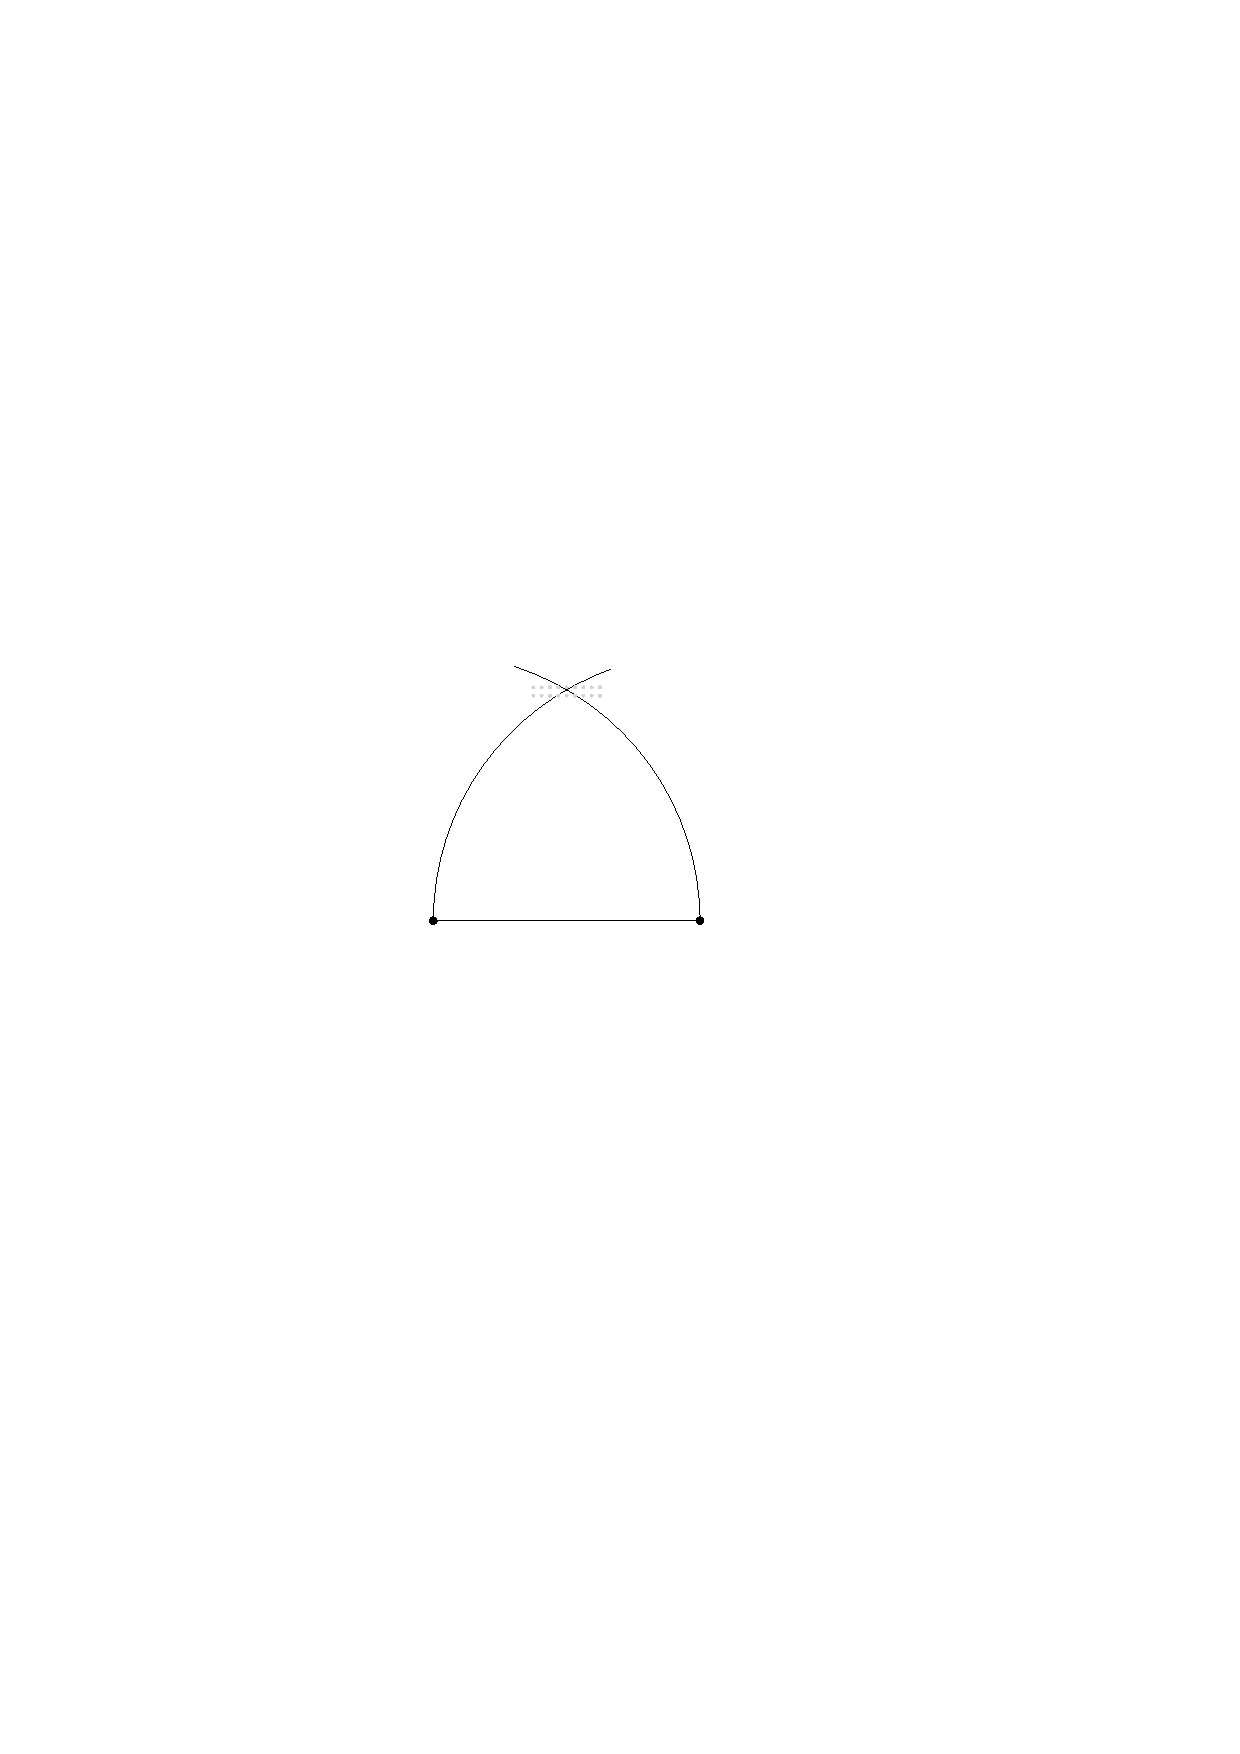
\includegraphics[width=0.7\textwidth,page=1]{drawings/small_example.pdf}
	\end{subfigure}
	\caption{There is no grid point for an optimal drawing without any bends}
\end{figure}

But, when introducing one bend per edge, there exists a drawing with an optimal ratio. 
\begin{figure}[H]
	\centering
	\begin{subfigure}{0.6\linewidth}
		\centering
		\includegraphics[width=0.7\textwidth,page=2]{drawings/small_example.pdf}
	\end{subfigure}
	\caption{With one bend, $K_3$ admits an optimal drawing}
\end{figure}
Allowing bends will help minimizing the ratio of a drawing. 